\documentclass{report}
\usepackage[margin=1in]{geometry}
\usepackage{setspace}
\usepackage{times}
\title{
	\textsc{ \small
		Washington State University \\
		School of Electrical Engineering and Computer Science \\
		EE 352, Electrical Engineering Laboratory
	} \\
	{\textsc{\small Lab \#4}} \\
	Non-ideal operational amplifier behavior
}

\author{
	Name: Kevin Evans \\
	Partner: Jacob Hnatiak
}
\date{Due Date: February 18, 2020}


% start sections at 1 with subsections to 1.1, 1.2...
\renewcommand{\thesection}{\arabic{section}}

%alias for vpp/rms
\newcommand{\pp}{_{pp}}
\newcommand{\rms}{_{rms}}
\newcommand{\Vpp}{\V\pp}
\newcommand{\Vrms}{\V\rms}

\usepackage{siunitx}
\usepackage{threeparttable}
\usepackage{booktabs}
\usepackage{multirow}
\usepackage{graphicx}
\usepackage{float}
\usepackage{amssymb,amsmath}
\begin{document}
\maketitle

\section*{Lab Overview}
% what was the lab about and the outcome?

The purpose of this lab was to explore the various real-world applications of op amps, specifically the OP27 op amp, and to gain an understanding of real-world limitations of the non-ideal characteristics of the amplifier. This lab specifically exposed us to the effects of open-loop gain bandwidth, slew rate distortion, offset measurements, and the common-mode rejection ratio (CMRR).

\section{Effects of open-loop gain bandwidth product}

\subsection{Purpose}
% purpose of the experiment and its specs and/or design requirements

The purpose of this experiment was to investigate the effects of the open-loop gain bandwidth the output voltage of the amplifier.

\subsection{Theoretical background}
% background and its theory of operation, circuit diagrams, the main equations, results from the prelab
The open-loop gain of a non-ideal opamp is dependent on the frequency as a first-order system with dc gain $A_0$ and cutoff frequency $f_b$. Generally, this gain is expressed as \begin{equation}
	A(jf) = \frac{A_0}{1 + jf / f_b}
\end{equation}
This can be approximated as the cutoff frequency $f_b$ is less than \SI{10}{\Hz}. As such, we can now express the gain as
\begin{equation}
	A(jf) \approx \frac{A_0 f_b}{jf} = \frac{f_t}{jf}
\end{equation}

If the gain-bandwidth product $f_t$ is known, we can estimate the cutoff frequency for the non-inverting amplifier, shown in Figure \ref{fig:exp1ckt} as
\begin{equation}
	f_0 = \frac{f_t}{1 + R_2 / R_1}
\end{equation}

\begin{figure}[h]
	\centering
	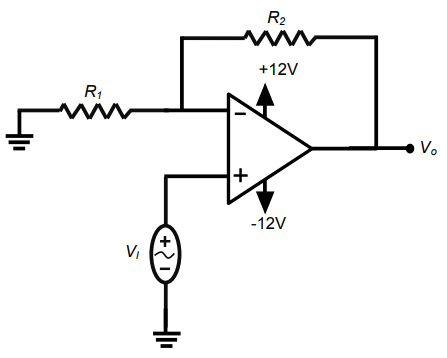
\includegraphics[width=0.5\linewidth]{exp1ckt}
	\caption{Circuit diagram of the non-inverting amplifier used in experiment 1.}
	\label{fig:exp1ckt}
\end{figure}

From the OP27 datasheet, the minimum and typical gain-bandwidth product is \SI{5.0}{\MHz} and \SI{8.0}{\MHz}. If $R_1$ is fixed as \SI{1}{\kohm}, then we can adjust $R_2$ to find the expected cutoff frequencies as shown in Table 
\ref{table:exp1gains} below.

\begin{table}[H]
	\centering
	\caption{Expected gains and cutoff frequencies of various $R_2$ configurations.}
	\label{table:exp1gains}
	\begin{threeparttable}
		\begin{tabular}{cccc}
			\toprule
			& & \multicolumn{2}{c}{Cutoff Frequency $f_0$} \\
			Gain (V/V) & $R_2$ & Minimum & Typical \\
			\midrule
			11 & \SI{10}{\kohm} & \SI{454}{\kHz} & \SI{727}{\kHz} \\
			48 & \SI{47}{\kohm} & \SI{104}{\kHz} & \SI{167}{\kHz}\\
			101 & \SI{100}{\kohm} & \SI{50}{\kHz} & \SI{74}{\kHz} \\
			\bottomrule
		\end{tabular}
	\end{threeparttable}
\end{table}

The first amplifier with \SI{11}{\V/\V} gain was simulated using OrCAD PSPICE, resulting in the response shown in Figure \ref{fig:exp1sim}.

\begin{figure}[H]
	\centering
	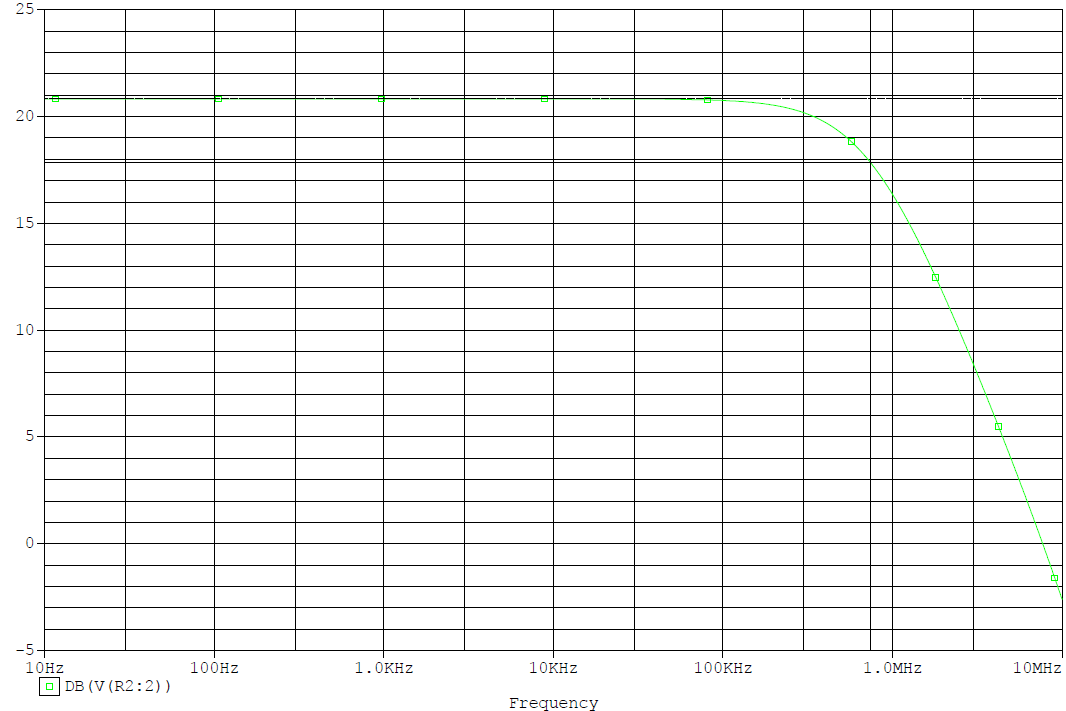
\includegraphics[width=0.7\linewidth]{exp1sim}
	\caption{Simulation of the 11 V/V amplifier}
	\label{fig:exp1sim}
\end{figure}

\subsection{Procedure}
The follow steps were carried out, as instructed by the lab assignment.
\begin{enumerate}
	\item The OP27 opamp was connected as a non-inverting amplifier using $R_2=\SI{10}{\kohm}$ (nominal) in the circuit shown in Figure \ref{fig:exp1ckt}.
	\item The function generator was attached to the input of the circuit and teed to CH1 of the oscilloscope. The output of the circuit was attached to CH2 of the oscilloscope.
	\item An input \SI{20}{\mV} (peak-to-peak) sine wave was generated at \SI{100}{\Hz} using the function generator.
	\item The input and output voltages were measured using the oscilloscope and the gain was recorded in Excel. As the frequency was low, this was assumed to be the dc gain.
	\item The frequency was increased slowly until it reached $\frac{G_{DC}}{\sqrt{2}} \approx 0.707 G_{DC}$. This was assumed to be the corner frequency. The gain-bandwidth product was calculated and recorded in the lab notebook.
	\item This data was plotted using Excel.
	\item Steps 2 through 5 were repeated for the \SI{47}{\kohm} and \SI{100}{\kohm} resistors.
\end{enumerate}

\subsection{Results and analysis}
% state all measured values, graphs, tables, and figs.
% state any deviation from theoretical expected values
% use tables and graphs
% * must justify error in results otherwise the experiment failed

\subsubsection{Measured component values}
The resistors were measured using the DMM and listed in Table \ref{table:exp1components}.

\begin{table}[h]
	\centering
	\caption{Experimental and nominal component values.}
	\label{table:exp1components}
	\begin{threeparttable}
		\begin{tabular}{clccc}
			\toprule
			\multicolumn{2}{c}{Component} & Nominal & Experimental & \% Error (Tolerance) \\
			\midrule
			$R_1$ & & \SI{1}{\kohm} & \SI{0.9728}{\kohm} & 2.7\% (5\%) \\
			$R_2$ & (11 V/V) & \SI{10}{\kohm} & \SI{9.743}{\kohm} & 2.6\% (5\%)\\
			$R_2$ & (48 V/V) & \SI{47}{\kohm} & \SI{46.42}{\kohm} & 1.2\% (5\%) \\
			$R_2$ & (101 V/V) & \SI{100}{\kohm} & \SI{99.48}{\kohm} & 0.5\% (5\%) \\
			\bottomrule
		\end{tabular}
	\end{threeparttable}
\end{table}

\subsubsection{Gain bandwidth values}
For each resistor, the gain bandwidth product was calculated and noted in Table \ref{table:exp1results} below. The average gain bandwidth product was \SI{5.65}{\MHz}, between the minimum and typical value expected in the datasheet. As this was in range, there is no error to be calculated in this experiment.

\begin{table}[H]
	\centering
	\caption{Gain bandwidth products of each resistor value.}
	\label{table:exp1results}
	\begin{threeparttable}
		\begin{tabular}{cccc}
			\toprule
			Nominal $R_2$ (Measured) & Gain & Cutoff frequency & Gain bandwidth product \\
			\midrule
			\SI{10}{\kohm} (\SI{9.743}{\kohm}) & \SI{10.8}{\V/\V} & \SI{825}{\kHz} & \SI{6.3}{\MHz} \\
			\SI{47}{\kohm} (\SI{46.42}{\kohm}) & \SI{48.4}{\V/\V} & \SI{162}{\kHz} & \SI{5.54}{\MHz} \\
			\SI{100}{\kohm} (\SI{99.48}{\kohm}) & \SI{102}{\V/\V} & \SI{71}{\kHz} & \SI{5.12}{\MHz} \\
			\bottomrule
		\end{tabular}
	\end{threeparttable}
\end{table}

\begin{figure}[h]
	\centering
	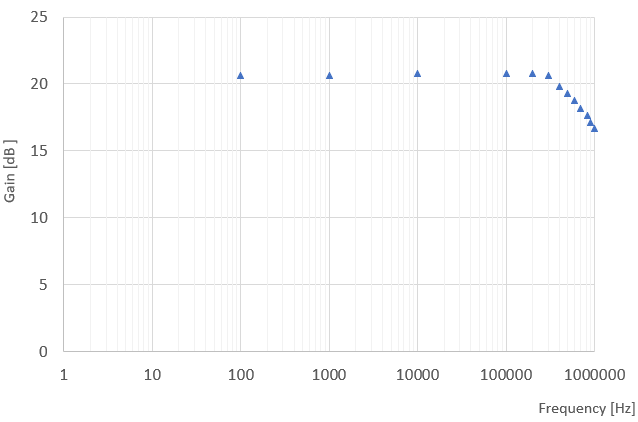
\includegraphics[width=0.7\linewidth]{exp1graph}
	\caption{Plot of the measured gain of the 11 V/V amplifier.}
	\label{fig:exp1graph}
\end{figure}


\subsection{Conclusion}
%  conclusion of the exp
The non-ideal characteristics were visible during this experiment as the bandwidth of the op amp was dependent on the frequency of the input signal attenuated the output gain. This was especially apparent at higher frequencies, acting as a low-pass filter before \SI{800}{\kHz}.


\section{Slew rate distortion}

\subsection{Purpose}
% purpose of the experiment and its specs and/or design requirements
Unlike ideal opamps, real-world opamps have limits on the output current and have an effective capacitance on the output of the amplifier. This provides some limitations on the apparent transfer characteristics of the amplifier.


%\subsection{Theoretical background}
% background and its theory of operation, circuit diagrams, the main equations, results from the prelab

\subsection{Procedure}
The follow steps were carried out, as instructed by the lab assignment.
\begin{enumerate}
	\item Using the OP27 opamp, a unity gain amplifier was constructed.
	\item The function generator was teed to CH1 of the oscilloscope and the input of the circuit.
	\item A \SI{0.1}{\V/\V} rectangular wave was applied using the function generator. The time/div was adjusted until the slew rate was clear and resulted in a ramping function to the steady-state voltage. Then, the slew rate was estimated.
	\item The estimated SR was compared to the expected datasheet SR value. The oscilloscope plot was saved to the flash drive.
	\item From the experimental SR value, $f_{max}$ was estimated for a sine wave with a \SI{1}{\V} (peak-to-peak) value. 
	\item A \SI{1}{\V} peak-to-peak sine wave was applied using the function generator. The frequency was increased until a distortion became evident on the output of the amplifier. The frequency was recorded.
\end{enumerate}

\subsection{Results and analysis}
% state all measured values, graphs, tables, and figs.
% state any deviation from theoretical expected values
% use tables and graphs
% * must justify error in results otherwise the experiment failed

%\subsubsection{Square wave response}
Using the square wave response, the time/div was adjusted until the slew became evident, as shown by Figure \ref{} below. The change in voltage and time was measured and used in the slope calculation, giving us the slew rate, \begin{align}
\Delta V & = \SI{19.2}{\mV} \notag \\
\Delta t & = \SI{0.0104}{\us}  \notag\\
SR & = \SI{1.8461}{\V/\us}
\end{align}
Relative to the datasheet value, this was found to be in range of the expected \num{1.2} to \SI{2.8}{\V/\us}. Next, a sine wave was applied and the frequency was adjusted until distortion became evident. Distortion was seen initially at \SI{600}{\kHz} and was very clear as it progressed up to \SI{700}{\kHz}. At \SI{600}{\kHz}, it was somewhat over the estimated and theoretical value of \SI{680}{\kHz}, but still in range of our expectations.

\subsection{Conclusion}
%  conclusion of the exp
This op amp had a clear slew rate, which was especially visible during the step response. The slew rate resulted in a slow ramp up to the unity signal. This was additionally visible in the sine response, albeit much less so: the distortion did not become evident until roughly \num{600} to \SI{650}{\kHz}. At higher frequencies, the signal became much more distorted, completely changing waveforms by \SI{700}{\kHz}, and becoming nearly triangular waves.

\section{DC Offset Voltage, DC Offset Current, DC Bias Current}

\subsection{Purpose}
% purpose of the experiment and its specs and/or design requirements
The purpose of this experiment was to find the offset voltage, current, and bias currents that are internal to the op amp. These values are a non-ideal characteristic contained with the operational amplifier that specifically are reflected in the inverting and non-inverting terminals.

%\subsection{Theoretical background}
% background and its theory of operation, circuit diagrams, the main equations, results from the prelab
\begin{figure}[h]
	\centering
	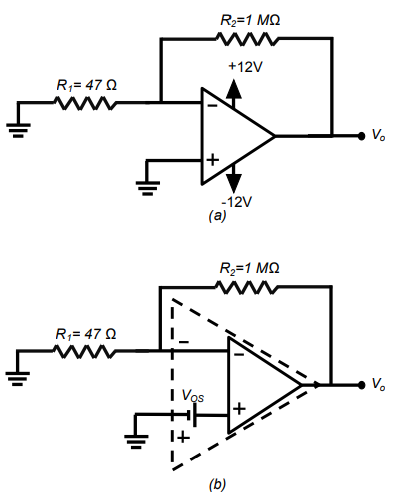
\includegraphics[width=0.5\linewidth]{exp3a}
	\caption{Circuits used in calculating the dc offset voltages.}
	\label{fig:exp3a}
\end{figure}

\begin{figure}[h]
	\centering
	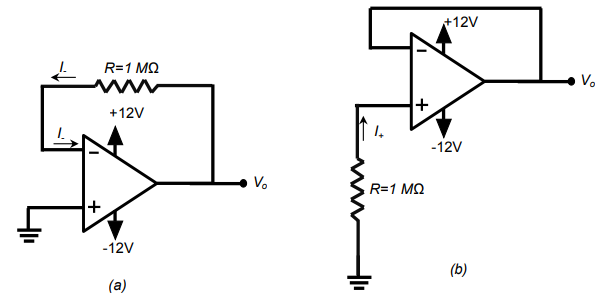
\includegraphics[width=0.7\linewidth]{exp3b}
	\caption{Circuit used in measuring the dc offset current.}
	\label{fig:exp3b}
\end{figure}
\begin{figure}[h]
	\centering
	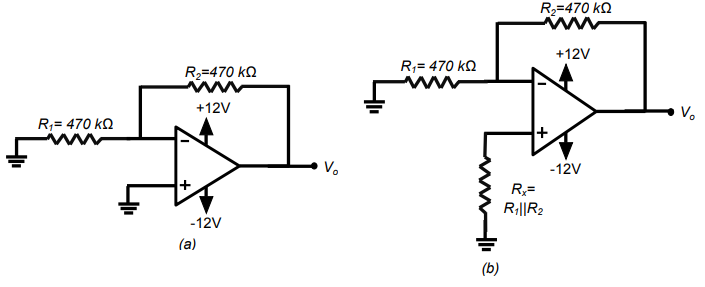
\includegraphics[width=0.7\linewidth]{exp3c}
	\caption{Circuit used in measuring the bias currents.}
	\label{fig:exp3c}
\end{figure}

\subsection{Procedure}
The follow steps were carried out, as instructed by the lab assignment.
\begin{enumerate}
	\item Estimate the input offset voltage 
		\begin{enumerate}
			\item The circuit shown in Figure \ref{fig:exp3a}(a) was constructed and the two resistor values were recorded. The output voltage was recorded using the DMM.
			
			\item From this, the offset voltage was estimated and compared to the typical and maximum offset voltage from the datasheet.
		\end{enumerate}
	
	\item Estimate the input bias currents and input offset currents.
		\begin{enumerate}
			\item The circuit shown in Figure \ref{fig:exp3b}(a) was constructed. The resistor value was recorded and the output voltage was measured using the DMM.
			\item The inverting current was estimated using this value using the offset voltage from Step 1.
			\item Then, Figure \ref{fig:exp3b}(b) was constructed and the output voltage was measured again.
			\item The non-inverting current was estimated similarly.
			\item From these values, the input bias and offset currents were estimated, then compared to the datasheet values.
		\end{enumerate}
	
	\item DC offset compensation circuit. \begin{enumerate}
		\item The circuit shown in Figure \ref{fig:exp3c} was constructed and the resistor values were recorded. The output voltage was measured using the DMM.
		\item Resistor $R_x$ was added to compensate for the offset measurement and the output voltage was measured again.
		\item The new output voltage was compared to the original uncompensated voltage.
	\end{enumerate}
\end{enumerate}

\subsection{Results and analysis}
% state all measured values, graphs, tables, and figs.
% state any deviation from theoretical expected values
% use tables and graphs
% * must justify error in results otherwise the experiment failed

\subsubsection{Measured component values}
\begin{table}[h]
	\centering
	\caption{Experimental and nominal component values.}
	\label{table:exp3components}
	\begin{threeparttable}
		\begin{tabular}{cccc}
			\toprule
			Component & Nominal & Experimental & \% Error (Tolerance) \\
			\midrule
			$R_1$ & \SI{47}{\ohm} & \SI{46.64}{\ohm} & \\
			$R_2$ & \SI{1}{\Mohm} & \SI{1.0149}{\Mohm} & \\
			\midrule
			$R$ & \SI{1}{\Mohm} & \SI{1.0149}{\Mohm} & \\
			\midrule
			$R_1$ & & & \\
			$R_2$ & & & \\
			$R_x$ & & &\\
			\bottomrule
		\end{tabular}
	\end{threeparttable}
\end{table}
The dc offset voltage was found to be \SI{38.25}{\uV}, in range of the data sheet. The currents $I_-$ and $I_+$ were found to be \SI{-0.386}{\nA} and \SI{0.362}{\nA}. From this, the bias current $I_B$ and offset current was found as \SI{73}{\nA}. Both of these exceed the specification from the datasheet, indicating this op amp has a particularly low bias current internally.

\subsection{Conclusion}
%  conclusion of the exp
The offset values of the OP27 amplifier were verified and our values were within the specifications listed in the datasheet. The input currents were fairly minimal, in the nano-ampere range, indicating a nearly-ideal behavior and minimal draw from the input. This is a desirable behavior and outperforms the typical range as listed in the datasheet.

\section{Common Mode Rejection Ratio (CMRR)}

\subsection{Purpose}
% purpose of the experiment and its specs and/or design requirements
In this experiment, the common mode rejection ratio was introduced, a number representing the ratio of the differential-to-common mode gain. Ideally, this number is infinite, indicating an ideal op amp.

%\subsection{Theoretical background}
% background and its theory of operation, circuit diagrams, the main equations, results from the prelab

\begin{figure}[h]
	\centering
	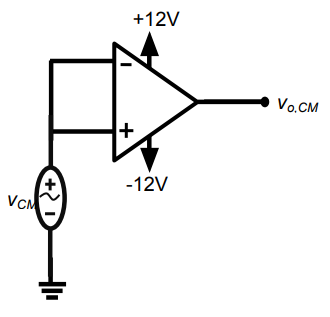
\includegraphics[width=0.4\linewidth]{exp4a}
	\caption{Circuit used to measure the common mode gain.}
	\label{fig:exp4a}
\end{figure}
\begin{figure}[h]
	\centering
	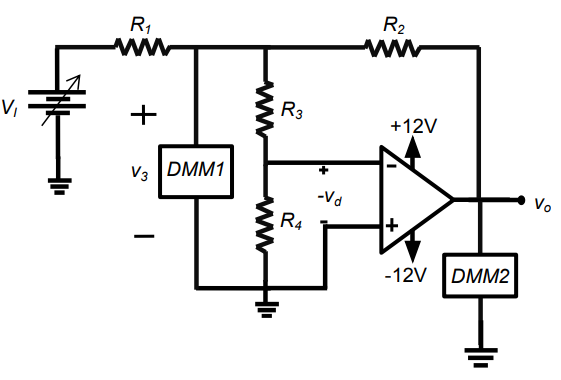
\includegraphics[width=0.5\linewidth]{exp4b}
	\caption{Circuit used in the second part of the CMRR experiment, allowing the differential gain to be calculated.}
	\label{fig:exp4b}
\end{figure}

\subsection{Procedure}
The follow steps were carried out, as instructed by the lab assignment.
\begin{enumerate}
	\item Measuring common mode gain $A_{cm}$
		\begin{enumerate}
			\item Using the OP27 op amp, the circuit shown in Figure \ref{fig:exp4a} was connected and a \SI{10}{\Vpp} sine wave was attached to both input terminals of the op amp.
			\item With the oscilloscope, the input and output terminals were measured and saved on the thumb drive.
			\item The common mode gain was calculated.
		\end{enumerate}
	\item Measuring the differential gain
		\begin{enumerate}
			\item Using the OP27 opamp, the circuit was connected as shown in Figure \ref{fig:exp4b}. The resistor values were measured using the DMM and recorded in the lab notebook. The input was set using the function generator at a low magnitude and the DC offset was varied.
			\item The DC offset was varied and the output voltage was measured using the DMM. The offset was adjusted until it reached \SI{9}{\Vpp}.
			\item The last step was repeated but the offset voltage was varied until it reached \SI{-9}{\Vpp}.
			\item The differential gain was calculated.
		\end{enumerate}
\end{enumerate}

\subsection{Results and analysis}
% state all measured values, graphs, tables, and figs.
% state any deviation from theoretical expected values
% use tables and graphs
% * must justify error in results otherwise the experiment failed

\subsubsection{Measured component values}
\begin{table}[h]
	\centering
	\caption{Experimental and nominal component values.}
	\label{table:lab2components}
	\begin{threeparttable}
		\begin{tabular}{cccc}
			\toprule
			Component & Nominal & Experimental & \% Error (Tolerance) \\
			\midrule
			$R_1$ & \SI{1}{\kohm} & \SI{0.9828}{\kohm} & \\
			$R_2$ & \SI{4.7}{\kohm} & \SI{4.547}{\kohm} & \\
			$R_3$ & \SI{47}{\kohm} & \SI{46.66}{\kohm} & \\
			$R_4$ & \SI{47}{\ohm} & \SI{46.24}{\ohm} & \\
			\bottomrule
		\end{tabular}
	\end{threeparttable}
\end{table}
The function generator was set to \SI{2}{\mV} (pp) as it was unable to reach the desired \SI{1}{\mV} (pp). The DMM read \SI{9.002}{\V} (dc) and the alternate DMM read \SI{8.95}{\mV}. Using this, the offset voltage was found to be \SI{-8.861}{\mV}. Next, the opposite voltage was found as \SI{14.95}{\mV}, resulting in an offset voltage of \SI{-1.480e-5}{\V}. 
The differential gain was found to be
\[ A_d = \SI{3030813.3}{\V/\V} = \SI{124.6}{\dB} \]
The CMRR was then found as
\[ CMRR = \num{1377642273} = \SI{182}{\dB} \]

\subsection{Conclusion}
%  conclusion of the exp
The CMRR found far exceeding the specification, of a minimum and typical value of 100 and 120 dB. This is notable as an ideal op amp would have an infinite CMRR. 
\end{document}